\section{Introdução}\label{introduuxe7uxe3o}

Com a crescente adoção de equipamentos IOT, como por exemplo o Raspberry
Pi que em quase 5 anos vendeu 10 milhões de unidades pelo mundo
\cite{raspberry-pi-blog:2016}, para monitoramento de sensores e
acionamento de cargas, cresce também a necessidade de ambientes de
acompanhamentos de tais medições. Para isso uma das melhores formas é
usar a nuvem para fazer o armazenamento, já que uma das caracteristicas
dos equipamentos IOT é o acesso a internet. Para atender essa
necessidade surge a ideia de criar um aplicativo web e livre que possa
captar informações destes dispositivos e que o acesso possa acontecer em
qualquer lugar.

\section{Objetivos}\label{objetivos}

O objetivo principal do \wm é fornecer uma \emph{api} leve, simples e
segura, visto que equipamentos IOT são limitados, para enviar e receber
informações da nuvem.

Para que haja melhor intercâmbio das informações tanto partindo do
equipamento IOT quanto chegando o protocolo de comunicação escolhido foi
o JSON, que segundo Douglas Crockford é um formato leve e de linguagem
independente para troca de informações \cite{crockford-2015}.

\section{Justificativa}\label{justificativa}

Sendo um aplicativo de código-fonte licenciado pela GPLv3 poderá ser
usado tanto para professores e alunos de cursos superiores e técnicos
para estudo de microcontroladores, sistemas embarcados e afins, como
para empresas ou pessoas que queiram interagir com seus equipamentos
pessoais.

A linguagem de programação escolhida foi o PHP, a qual é fácil de
aprender, normalmente lecionada em cursos superiores e técnicos e de
hospedagem barata.

Outra característica a ser levada em conta é a forma de autenticação.
Uma autenticação convencional envolve a troca de \emph{cookies} entre
servidor e cliente, além de espaço em disco para guardar tais
informações. Em sistemas IOT que se supoem que possam crescer de forma
rápida, ou seja, o número de equipamentos pode aumentar, é necessário um
sistema de autenticação capaz de ser escalável mesmo em condições
limitadas. Para isso foi utilizado o padrão JWT (ou \emph{JSON Web
Tokens}), que é um padrão aberto (RFC 7519 \cite{rfc7519-2015}) que
define uma maneira compacta e auto-contida de transmitir de forma segura
informações entre pares através de um objeto JSON \cite{jwt-2016}. Esta
informação pode ser verificada e confirmada pois é assinada
digitalmente. Informações JWT podem ser assinadas usando um segredo (com
o algoritmo HMAC \cite{rfc2104-1997}) ou um par de chave pública e
privada usando RSA \cite{rfc3447-2003}.

\begin{figure}[h]
    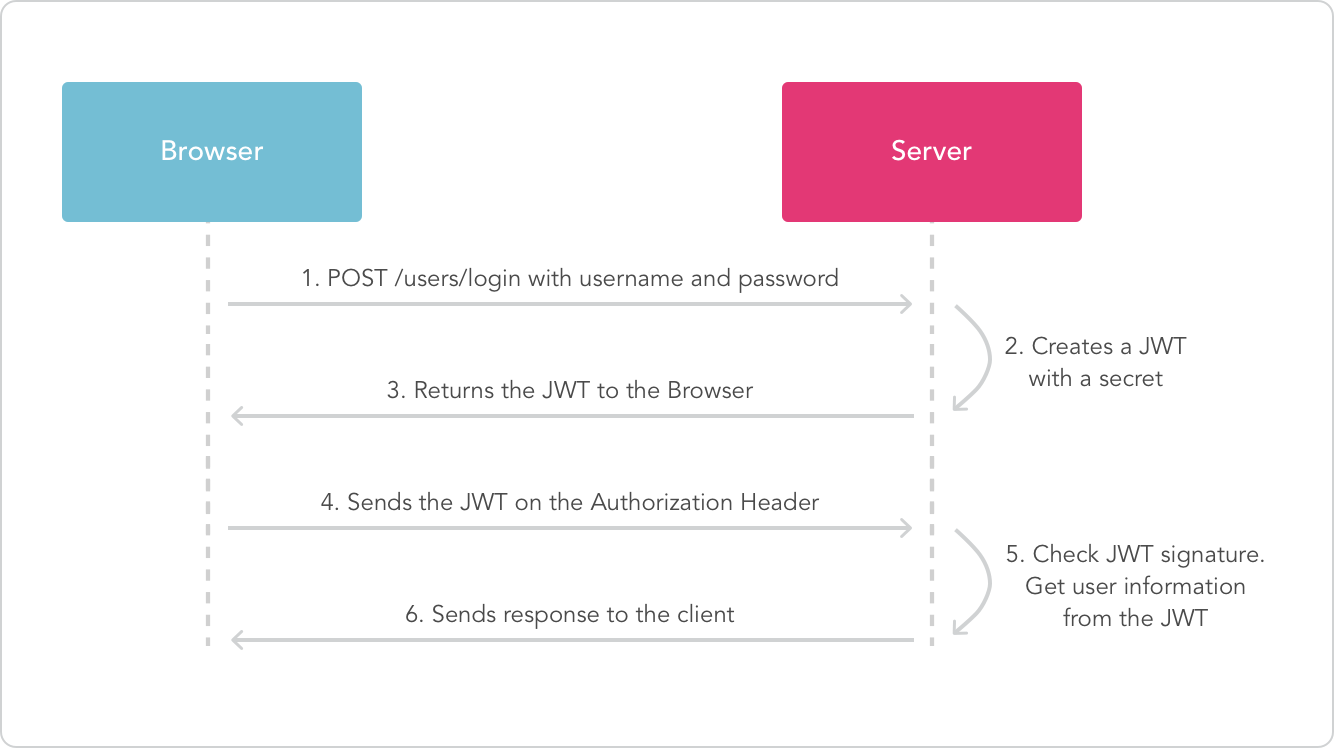
\includegraphics[scale=0.3]{img/jwt-diagram.png}
    \caption{Diagrama do processo de autenticação - Fonte: https://cdn.auth0.com/content/jwt/jwt-diagram.png}
\end{figure}

\section{Revisão Teórica}\label{revisuxe3o-teuxf3rica}

Muitas são as soluções de monitoramento de equipamentos IOT, desde
grandes empresas como Oracle, Amazon, Google, Microsoft; até soluções
livres como Kaa, ThingSpeak, macchina.io, SiteWhere
\cite{postscapes-iot-2016}.

O grande desafio é permitir a extensão da ferramenta para necessidades
específicas. Ferramentas com o Kaa permitem criar módulos próprios,
sistemas de análises e modelo de dados, fazendo com que a ferramenta se
adapte ao que você precisa \cite{kaa-2014}.

De forma semelhante outras ferramentas como macchina.io oferecem opções
de criar \emph{bundles} \cite{macchina.io-2016}, o ThingSpeak oferece
opção de criar \emph{apps}, que podem envolver visualização em gráficos
e tomada de decisões \cite{thingspeak-2016}.

Nesse sentido a ferramenta proposta possui um sistema de plugins, que
são desenvolvidos como \emph{Laravel Packages}
\cite{laravel-packages-2016}. Cada nova funcionalidade é criada através
da ferramenta \emph{Laravel} e pode ser desenvolvida e habilitada
localmente.

A proposta é ter uma tela de acompanhamento dos dados captados do
equipamento e a visualizaçãos ser específica. A documentação em
português do brasil para criar um novo plugin pode ser encontrada em
\url{https://sanusb-grupo.github.io/wireless-monitor/pt-br/plugin-development.html}.

\subsection{Comparativo com outras ferramentas
livres}\label{comparativo-com-outras-ferramentas-livres}

\begin{longtable}[c]{@{}llll@{}}
\toprule\addlinespace
\begin{minipage}[b]{0.22\columnwidth}\raggedright
Aplicativo
\end{minipage} & \begin{minipage}[b]{0.28\columnwidth}\raggedright
Ambiente do Servidor
\end{minipage} & \begin{minipage}[b]{0.25\columnwidth}\raggedright
Suporte a plugins
\end{minipage} & \begin{minipage}[b]{0.12\columnwidth}\raggedright
SDK
\end{minipage}
\\\addlinespace
\midrule\endhead
\begin{minipage}[t]{0.22\columnwidth}\raggedright
Kaa
\end{minipage} & \begin{minipage}[t]{0.28\columnwidth}\raggedright
Java
\end{minipage} & \begin{minipage}[t]{0.25\columnwidth}\raggedright
Sim
\end{minipage} & \begin{minipage}[t]{0.12\columnwidth}\raggedright
Sim
\end{minipage}
\\\addlinespace
\begin{minipage}[t]{0.22\columnwidth}\raggedright
macchina.io
\end{minipage} & \begin{minipage}[t]{0.28\columnwidth}\raggedright
C++/NodeJS
\end{minipage} & \begin{minipage}[t]{0.25\columnwidth}\raggedright
Sim
\end{minipage} & \begin{minipage}[t]{0.12\columnwidth}\raggedright
Sim
\end{minipage}
\\\addlinespace
\begin{minipage}[t]{0.22\columnwidth}\raggedright
SiteWhere
\end{minipage} & \begin{minipage}[t]{0.28\columnwidth}\raggedright
Java
\end{minipage} & \begin{minipage}[t]{0.25\columnwidth}\raggedright
Sim
\end{minipage} & \begin{minipage}[t]{0.12\columnwidth}\raggedright
Sim
\end{minipage}
\\\addlinespace
\begin{minipage}[t]{0.22\columnwidth}\raggedright
ThingSpeak
\end{minipage} & \begin{minipage}[t]{0.28\columnwidth}\raggedright
Ruby
\end{minipage} & \begin{minipage}[t]{0.25\columnwidth}\raggedright
Sim
\end{minipage} & \begin{minipage}[t]{0.12\columnwidth}\raggedright
Sim
\end{minipage}
\\\addlinespace
\begin{minipage}[t]{0.22\columnwidth}\raggedright
Wireless Monitor
\end{minipage} & \begin{minipage}[t]{0.28\columnwidth}\raggedright
PHP
\end{minipage} & \begin{minipage}[t]{0.25\columnwidth}\raggedright
Sim
\end{minipage} & \begin{minipage}[t]{0.12\columnwidth}\raggedright
Não
\end{minipage}
\\\addlinespace
\bottomrule
\end{longtable}

\section{Arquitetura}\label{arquitetura}

É necessário um Servidor, um equipamento IOT, seja ESP8266 ou Raspberry
Pi com Arduino; e um navegador de internet no cliente.

A arquitetura segue o modelo da Figura \ref{fig:arquitetura}.

\begin{figure}[h]
    \centering
    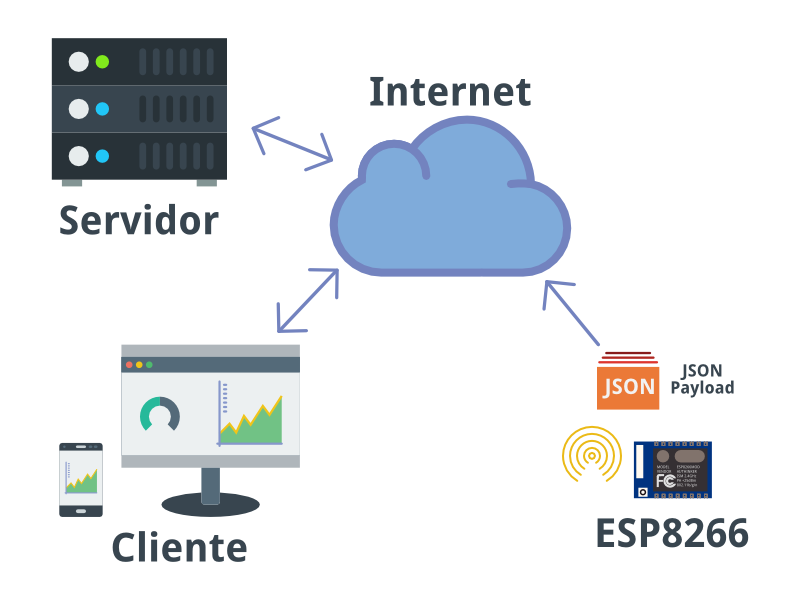
\includegraphics[scale=0.45]{img/arquitetura.png}
    \caption{Arquitetura} \label{fig:arquitetura}
\end{figure}

\section{Aplicação}\label{aplicauxe7uxe3o}

Vejamos um passo a passo de como o aplicativo funciona.

\subsection{Cadastro do desenvolvedor}\label{cadastro-do-desenvolvedor}

O desenvolvedor inicialmente deve fazer um cadastro simples na
ferramenta. Esse cadastro irá criar para ele uma \texttt{api\_key}, ou
seja, uma chave única no formato UUID 4 \cite{rfc4122:2005}.

\subsection{Criar um \emph{Monitor}}\label{criar-um-monitor}

Um \emph{Monitor} é um componente interno do sistema criado pelo
desenvolvedor de acordo com sua necessidade, é o instrumento que
caracteriza os dados coletados e os apresenta na interface web.

Imagine que o desenvolvedor queira medir a temperatura de um ambiente e
acompanhar suas variações. Para isso ele deve criar um \emph{Monitor} de
Temperatura, que apenas recebe um valor a um certo intervalo de tempo.
Dessa forma o desenvolvedor pode acompanhar as variações ou ainda ver em
forma de gráfico um conjunto de variações de um período de tempo
anterior.

Da mesma forma que uma chave UUID é criada para o desenvolvedor, uma
chave é criada para o Monitor - \texttt{monitor\_key}.

\subsection{Autenticação do
equipamento}\label{autenticauxe7uxe3o-do-equipamento}

Para autenticar e identificar o desenvolvedor e seu \emph{monitor} é
preciso enviar a \texttt{api\_key} e a \texttt{monitor\_key} via método
\emph{POST} para o \emph{endpoint} \texttt{/api/authenticate}. Em caso
positivo o sistema irá retornar um \emph{token}. Esse \emph{token}
servirá para qualquer troca de informações futuras entre o equipamento
IOT e o sistema. Esse método de autenticação é chamado de JWT ou
\emph{JSON Web Token}, um padrão internacional \emph{RFC 7519} para
intercâmbio de dados entre entidades.

Após ter o \emph{token} o desenvolvedor deve passá-lo através da
\emph{Header HTTP} denominada \emph{Authorization} usando \emph{schema
Bearer}. Algo do tipo:

\begin{verbatim}
Authorization: Bearer <token>
\end{verbatim}

Um \emph{token} é formado pelas seguintes informações:

\begin{itemize}
\itemsep1pt\parskip0pt\parsep0pt
\item
  \emph{Header}
\item
  \emph{Payload}
\item
  \emph{Signature}
\end{itemize}

Essa é uma forma segura e com pouco custo de memória. Além de ser uma
forma de autenticação \emph{stateless}, em que não são usadas sessões e
nem mesmo \emph{cookies}.

\subsection{Envio dos dados}\label{envio-dos-dados}

Além do cabeçalho contendo o \emph{token} o usuário deve passar os
valores coletados pelo equipamento e enviar para o sistema. Para isso
ele deve enviar uma requisição \emph{POST} para o \emph{endpoint}
\texttt{/api/send}, com o atributo \texttt{data} contendo um JSON com os
dados.

No exemplo do \emph{Monitor} de temperatura é necessário enviar apenas o
valor, algo do tipo:

\begin{verbatim}
{
    "value": 23.89
}
\end{verbatim}

\subsection{Descrição dos
componentes}\label{descriuxe7uxe3o-dos-componentes}

Neste tópico são descritos os componentes e as ferramentas utilizadas
para o desenvolvimento e uso do plugin de Temperatura.

\subsubsection{Sistema embarcado linux}\label{sistema-embarcado-linux}

Foi utilizado a plataforma Raspberry Pi como sistema embarcado, que irá
servir para cominucação com o Servidor e o dispositivo de captura de
temperatura.

\subsubsection{Microcontrolador}\label{microcontrolador}

A plataforma Arduino foi escolhida para servir de ponte entre o
componente de medição de temperatura e o sistema embarcado.

\subsubsection{Sensor de temperatura}\label{sensor-de-temperatura}

Como sendor de temperatura foi usado o LM35 da Texas Instruments. A
série LM35 é composta de dispositivos de circuito integrado para medição
de temperatura com a tensão de saída linearmente proporcional a
temperatura em graus Celcius. O sensor LM35 tem a vantagem sobre
sensores de temperatura linear calibrados em Kelvin, devido a não ser
necessário subtrair uma alta tensão constante da saída para obter uma
escala conveniente \cite{lm35:2016}.

\subsection{Ambiente de execução}\label{ambiente-de-execuuxe7uxe3o}

Para esse exemplo o ambiente de execução escolhido foi o NodeJS, que é
um envólucro (\emph{wrapper}) do ambiente de execução JavaScript de alta
performance chamado V8 usado no navegador Google Chrome. O Node permite
que o V8 funcione em contextos diferentes do browser, na maioria das
vezes fornecendo APIs adicionais que são otimizadas para casos
específicos \cite{hughes-croucher:2012}. Por exemplo no caso de
equipamentos IOT é perfeito, pois se trata de um dispositivo orientado a
eventos, assim como o NodeJS.

Para auxiliar na conversação entre o NodeJS e o Arduino foi usado a
ferramenta Johnny-Five, uma plataforma livre Javascript para Robôs e IOT
\cite{johnny-five:2012}.

\subsection{Princípios de
execução}\label{princuxedpios-de-execuuxe7uxe3o}

O NodeJS deve ser instalado no Raspberry Pi já que possui suporte a
arquitetura ARM. Um projeto NodeJS deve ser criado tendo como
dependências o Johnny-Five e uma biblioteca de resquisições HTTP, como
por exemplo request \cite{request:2016}. Dessa forma o Johnny-Five se
encarregará de se comunicar com o Arduino requisitando a temperatura do
componente LM35. Com a resposta em mãos o NodeJS irá enviar as medições
ao Servidor.

\subsection{Visualização dos dados}\label{visualizauxe7uxe3o-dos-dados}

Após captar e enviar dados do IOT para a nuvem é possível acompanhar os
resultados pelo sistema. A forma de visualização será como mostra a
Figura \ref{fig:view-monitor}.

\begin{figure}[h]
    \centering
    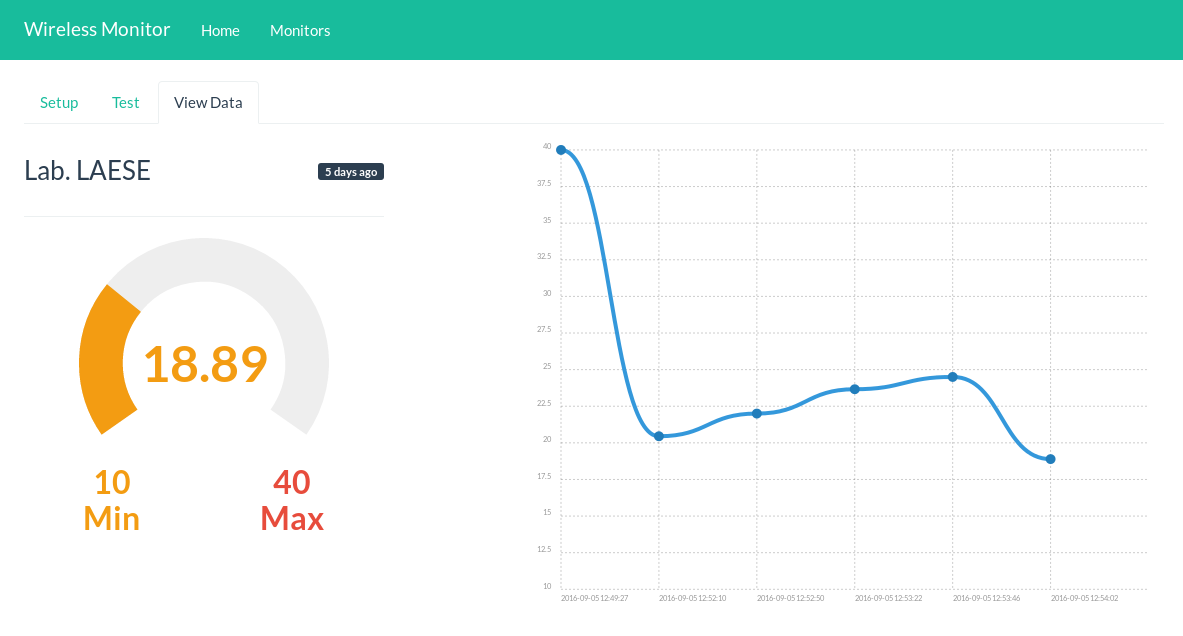
\includegraphics[scale=0.35]{img/temperature-show.png}
    \caption{Visualização dos dados na web} \label{fig:view-monitor}
\end{figure}
